\section{Band Limited Space with Rational Sampling Rate Changes}\label{sec:p2}
\begin{enumerate}[(a)]
\item Since we only care about the effect of $g$, we consider only until $g[n]$ is apply (the first 5 steps). 

Figure \ref{fig:p2-1} shows the results for $M=2, N=3, K=3$. After upsampling by 2 (second row), we need the cut-off frequency of $g$ to be $\frac{\pi}{3} \leq w_c \leq \frac{\pi}{3}$. By applying the low-pass filter $g[-n]$ (third row), the gap between two copies is $\frac{5\pi}{3} - \frac{\pi}{3} = \frac{4\pi}{3}$. After downsampling by 3 (forth row), the gap is reduced to 0, so upsampling it by 3 (fifth row) also gives the same gap. So the cut-off frequency has to be $w_c = \frac{\pi}{3}$.

\begin{figure}
	\centering
	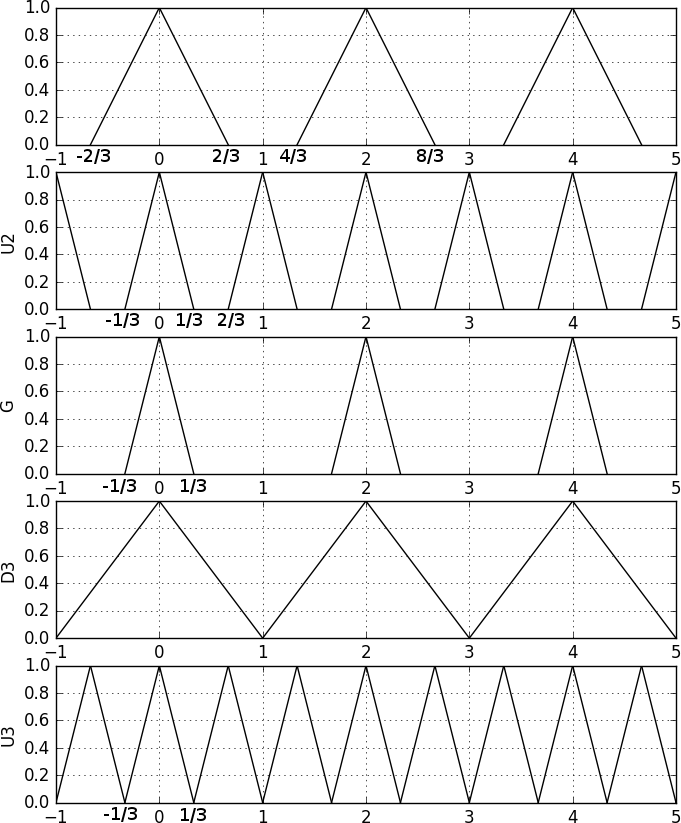
\includegraphics[width=\textwidth]{images/p2-1}
	\caption{$M=2, N=3, K=3$ ($x$ scale is $\pi$)}
	\label{fig:p2-1}
\end{figure}

\item Figure \ref{fig:p2-2} shows the results for$M=2, N=3, K=4$. After upsampling by 2 (second row), we need the cut-off frequency of $g$ to be $\frac{\pi}{4} \leq w_c \leq \frac{3\pi}{4}$. After apply downsampling by 3 (forth row), the gap is $\frac{\pi}{2}$. Therefore the gap is reduced by a third after upsampling by 3 (fifth row). So the second condition for cut-off frequency is $\frac{\pi}{4} \leq w_c \leq \frac{5\pi}{12}$. 
\[\frac{\pi}{4} \leq w_c \leq \frac{3\pi}{4} \text{ and } \frac{\pi}{4} \leq w_c \leq \frac{5\pi}{12} \Rightarrow \frac{\pi}{4} \leq w_c \leq \frac{5\pi}{12}\]
\begin{figure}
	\centering
	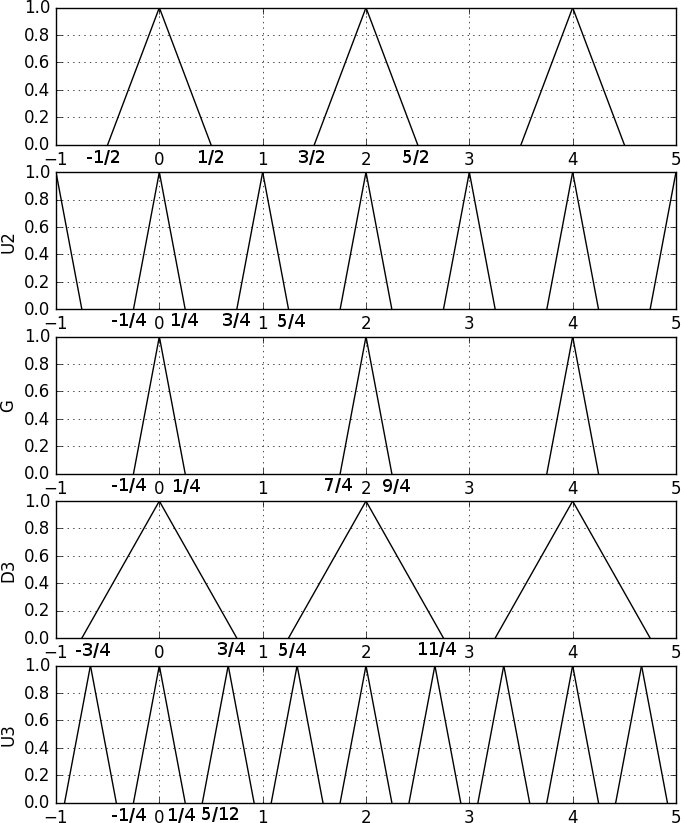
\includegraphics[width=\textwidth]{images/p2-2}
	\caption{$M=2, N=3, K=4$ ($x$ scale is $\pi$)}
	\label{fig:p2-2}
\end{figure}

\item If the signal in $[-\frac{2\pi}{K},\frac{2\pi}{K}]$, the gap's width is 
\[2\pi - \frac{2\pi}{K} -\frac{2\pi}{K} = 2\pi(1-\frac{2}{K})\]
After upsampling by $M$, the range is $[-\frac{2\pi}{KM},\frac{2\pi}{KM}]$ and the gap is $\frac{2\pi}{M} (1-\frac{2}{K})$. Therefore the first condition of $w_c$ is 
\[\frac{2\pi}{KM} \leq w_c \leq \frac{2\pi}{KM} + \frac{2\pi}{M} (1-\frac{2}{K}) \Leftrightarrow \frac{2\pi}{KM} \leq w_c \leq \frac{2\pi}{M} (1-\frac{1}{K})\]
After downsampling by $N$, the $[-\frac{2\pi N}{KM},\frac{2\pi N}{KM}]$ and the gap is $2\pi - \frac{2\pi N}{KM} - \frac{2\pi N}{KM} = 2\pi(1-\frac{2}{KM})$.

Therefore, after upsampling by $N$, the lower bound of the first copy (after at frequency of 0) is
\[\frac{1}{N} \cdot \frac{2\pi N}{KM} + \frac{1}{N}\cdot 2\pi(1-\frac{2N}{KM}) = \frac{2\pi}{KM} + \frac{2\pi}{N} - \frac{4\pi}{KM} = \frac{2\pi}{N} - \frac{2\pi}{KM} = 2\pi(\frac{1}{N} - \frac{1}{KM})\]

So the second condition of $w_c$ is
\[ \frac{2\pi}{KM} \leq w_c \leq 2\pi(\frac{1}{N} - \frac{1}{KM}) \]
Combining the first and second condition gives
\[ \frac{2\pi}{KM} \leq w_c \leq 2\pi(\frac{1}{N} - \frac{1}{KM}) \qquad (\because M<N\text{ so the second condition is tighter})\]
\end{enumerate}